\documentclass[12pt]{article}
\usepackage[english]{babel}
\usepackage[utf8x]{inputenc}
\usepackage{amsmath}
\usepackage{graphicx}
\usepackage[colorinlistoftodos]{todonotes}

\begin{document}

\begin{titlepage}

\newcommand{\HRule}{\rule{\linewidth}{0.5mm}} 

\center
 


\includegraphics{university_logo1.jpg} \\ [1cm]
\textsc{\LARGE Syracuse University}\\[1cm] 


\HRule \\[0.8cm]
{ \huge \bfseries Twitter Sentiment Analysis with Geographic Visualization}\\[0.4cm] 
\HRule \\[1.4cm]
 

\begin{minipage}{0.5\textwidth}
\begin{flushleft}
\emph{Author:}\\
Chetanraj \textsc{Kadam} - 250256631 \\
Pushkar \textsc{Tatiya} - 212517742 \\
Sakshi \textsc{Salokhe} - 201026946\\
Varun \textsc{Mulay} - 721214633 
\end{flushleft}
\end{minipage}
~
\begin{minipage}{0.4\textwidth}
\begin{flushright} \large
\emph{Professor:} \\
Martin \textsc{Harrison} 
\end{flushright}
\end{minipage}\\[1cm]
{\today}\\[0.8cm]

\vfill 

\end{titlepage}
\tableofcontents
\newpage


\begin{abstract}
The application is designed in order to provide sentimental analysis of tweets related to a particular hashtag and to display parts of the world or a particular area did most of the tweets come from. The homepage will display the top 10 trending hashtags. From the displayed 10 hashtags, the user can click on any hashtag of his choice. Based on the hashtag chosen, all the tweets related to that particular hashtag will be extracted. Sentimental Analysis is performed on the extracted tweets to find if the tweets are positive, negative or neutral. After performing Sentiment Analysis, the location tag of each tweet which were extracted, will be used to plot locations of the tweets over the map with different colours for positive, negative and neutral sentiments.
\vfill
\end{abstract}
\newpage
\section{Introduction}

Sentiment Analysis is the process of determining the emotional tone behind a series of words, used to gain an understanding of the the attitudes, opinions and emotions expressed within an online mention. It  is extremely useful in social media monitoring as it allows us to gain an overview of the wider public opinion behind certain topics. The applications of sentiment analysis are broad and powerful. The ability to extract insights from social data is a practice that is being widely adopted by organisations across the world. Shifts in sentiment on social media have been shown to correlate with shifts in the stock market. 
Few real life examples of Sentiment Analysis being applied are:
The Obama administration used sentiment analysis to gauge public opinion to policy announcements and campaign messages ahead of 2012 presidential election.

The ability to quickly understand consumer attitudes and react accordingly is something that Expedia Canada took advantage of when they noticed that there was a steady increase in negative feedback to the music used in one of their television adverts.

In the similar way, the application that we have developed will be used to do sentiment analysis over tweets. The basic motive of this application is to find out the sentiment analysis of  tweets for a particular hashtag and to find out the region where these tweets came from based on their categories (Positive, Negative and Neutral).
The advantage of this application is to give the user the flexibility to choose hashtag from the top trending ones and select the number of tweets that he wants to analyse.
\newpage

\section{Specifications}

\subsection{Source of data}

We used data extracted from twitter which included the tweets, user location and coordinates of the user who tweeted.
\subsection{API used}
We used twitter app API for extraction of Twitter data and Google maps API to plot the coordinates on the map. 

\subsection{Libraries used}
\begin{enumerate}
\item Tweepy
\item Pandas
\item Textblob
\item Numpy
\item Geocoder
\item Bokeh
\end{enumerate}
\newpage

\section{Algorithm}
\begin{enumerate}
\item  We use TextBlob for sentiment analysis which is built on the basis of Naive Bayes algorithm. 
\item TextBlob breaks the tweet into words and Naive Bayes algorithm processes every word and assigns polarity to the tweets.
\item If the polarity of the word is greater than 0 (polarity > 0), then the word is considered to be Positive. \\ \\
If the polarity of the word is equal to 0 (polarity = 0), then the word is considered to be Neutral.\\ \\
If the polarity of the word is less than 0 (polarity < 0), then the word is considered to be Negative.
\item Naive Bayes works on the basis of the formula :
\[ P(X \mathbin{\vert} c) =\frac {P(c \mathbin{\vert} X) \hspace{0.2cm} P(c)}{P(X)}\]
\item Use of Pandas to read and write the data into csv file.
\item Bokeh and Google maps API was used for plotting the coordinates on the map along with colors assigned according to the sentiment for the tweet.

\end{enumerate}
\newpage
\section{Procedure}
\begin{enumerate}
\item When the program is executed, the user will get a list of top 10 trending hashtags for that particular day.
\item User can select the hashtag and number of tweets for that hashtag for which he wants to perform the analysis.
\item Sentiment Analysis will be performed on the data extracted. A pie chart is shown denoting the percentage positive, negative and neutral tweets. The information about the sentiment for every tweet is maintained in a CSV file.
\item Location data is extracted for every tweet and stored in the form of latitude and longitude.
\item The CSV file containing the latitude, longitude and sentiment label is then plotted on the map to get the final output.
\end{enumerate}
\newpage
\section{Output}
\textsc{Top 10 trending hashtags and user input}\\[0.5cm]
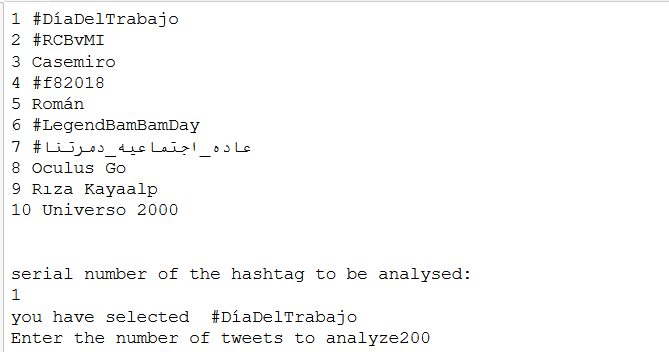
\includegraphics{Output_1.PNG} \\ [2cm]
\newpage
\textsc{Sentiment Analysis on the selected hashtag }\\[0.5cm]
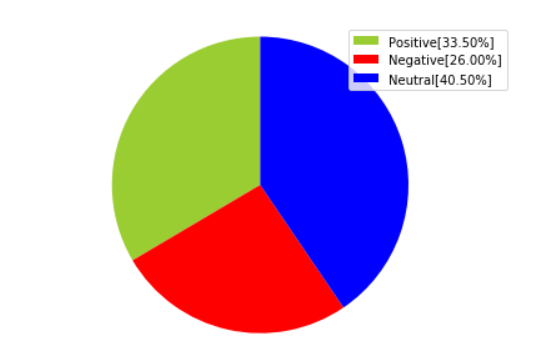
\includegraphics{Output_2.PNG} \\ [2cm]
\newpage
\textsc{Plotting on the map}\\[0.5cm]
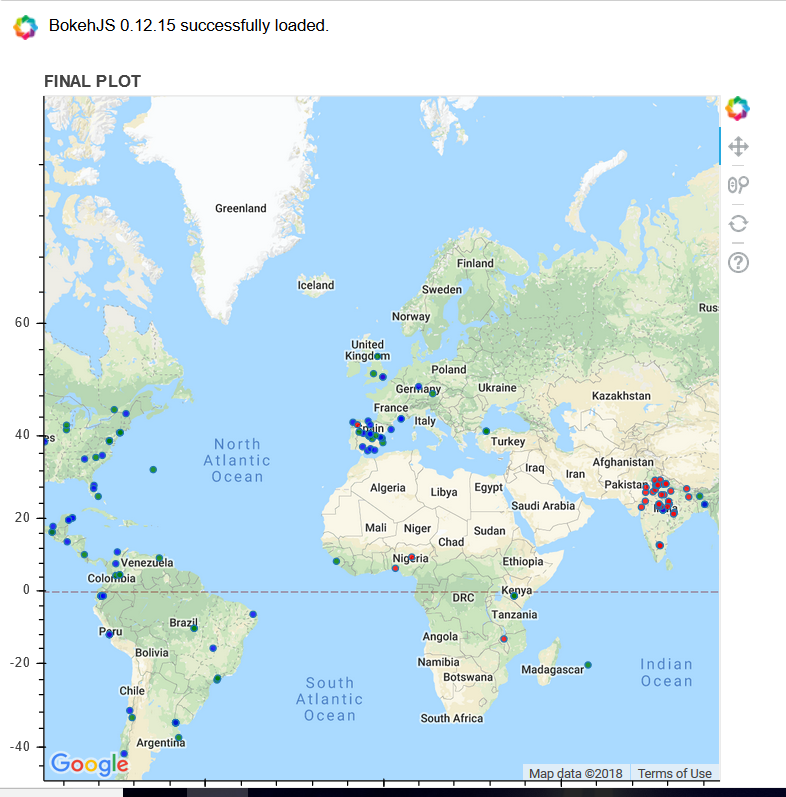
\includegraphics{Output_3.PNG} \\ [2cm]

\section{Conclusions}
Geographic visualization allows visual access to huge amounts of data which is otherwise hard to analyze. Data visualization gives us easily digestible visuals by
providing the main gist of the huge amount of data on a particular topic.
In particular, geographic visualization helps you understand trends, patterns and to make correlations. This type of visualization provides regional quantitative information.
This project aims to scrape tweets data of trending hashtags
and map them these tweets by their geographic location on the
world map. Also, additionally, we do sentiment analysis on these
hashtags and present it on a pie chart.

\newpage
\section{Major Contribution:}
During the process of building the project, the task of extraction of top trending tweets and extracting the top 10 out of them and displaying it and taking user input was done by Pushkar Tatiya and Sakshi Salokhe. The sentiment Analysis part of the project was done by Varun Mulay. The task of plotting the location data on google maps by preprocessing the stored data was done by Chetanraj Kadam, Pushkar Tatiya and Sakshi Salokhe.
The task of integrating the project and the documentation part was done by all the team members collectively.


\newpage
\begin{thebibliography}{9}
\bibitem{Geocode website} 
Visualizing Geocode Data
\\\texttt{http://support.gnip.com/articles/visualizing-twitter-geo-data.html}
 
\bibitem{extractwebsite}
Extract data from twitter
\\\texttt{http://www.mikaelbrunila.fi/2017/03/27/scraping-extracting-mapping-geodata-twitter/}
 
\bibitem{bokehwebsite} 
Plotting the data on map.
\\\texttt{https://bokeh.pydata.org/en/latest/docs/user\_guide/geo.html}
\end{thebibliography}



\end{document}